
\chapter{Feed Forward Neural Network in C++ 17 and OpenMP for performance optimization}

\section{Abstract}


In the project for course ECE 572, I will implement a feed forward neural network with sigmoid activation function. 

\section{Introduction}

Artificial Neural Networks (ANNs) are used in wide range of applications including system modeling and identification, signal processing, image processing, control systems and time series forecasting. The baseline of those models is a special class called Feed Forward Neural Network\cite{bebis1994nns,murat2006overview}. In this subclass of models, data is propagated forward only, and the model parameters are grouped in layers with no intra-communication. There is theoretically an infinite number of possible architecture regarding this type of models, hence they can have a lot of layers. In fact, Feed Forward Neural Networks were the beginning of a new Artificial Intelligence (AI) sub-field called Deep Learning, where the models used are designed to capture complicated patters. For that purpose, the model architecture as well as the dataset used to train them is very large. Consequently, in such cases the model performance poses a substantial challenge. There are several attempts on efficient ANN implementation using techniques, such as parallelization, to exploit the computational capabilities of the system architecture running a model\cite{huqqani2013multicore}. Using low-level programming languages, such as C++\cite{stourstrup2013cpp}, and frameworks that enable advanced parallelization and efficient data handling techniques, such as OpenMP\cite{dagum1998openmp}, the programmer can achieve better results in terms of performance compared to most state-of-the-art Deep Learning frameworks\cite{Jang2008NeuralNI}. 

\par

For the project of course ECE 572, I will try to implement a feed forward model with sigmoid activation function. The user will have to make little to no configurations before the execution of the driver. It will be fully re-configurable regarding the architecture of the model. For example, the user will be able to define the layers and number of neurons using command line arguments. Moreover, the software architecture will follow that of well known deep learning frameworks, such as PyTorch\cite{paszke2019pytorch}. That way the user will be able to easily navigate around the project if there is some prior experience with such frameworks. Furthermore, the user will be kept well informed throughout the data loading, the training and the inference process with \textit{progress bars}. Finally, the advantages of the proposed project will be demonstrated using a well known dataset, Fashion MNIST\cite{FashionMNIST2017Xiao}.

\section{Challenges}

The implementation of a neural network in theory is an easy process. However, when it comes to putting together those formulas using software, the engineer is challenged to compile an efficient code implementation. The challenge becomes even greater when the project is carried out in a low-level programming language, such as C++, where the engineer has to solve substantial numerical and challenges since the project is based on scientific computation. After solving those challenges, the engineer has to structure the code in order to implement parallel software architectures and data pipelining for efficient execution. In this project, the optimization part will utilize the OpenMP framework for software parallelization and extreme device utilization.

\section{Comparison}

To actually realize the magnitude of optimization achieved by the parallel version of the project, I've implemented $2$ more versions. The first is the \textit{Python} version using \textit{PyTorch}, which is the fastest deep learning framework in Python. The second is a \texttt{C++} implementation of the proposed feed forward neural network model running in serial mode. The \textit{Python} version was implemented to capture the performance gap compared to the \texttt{C++} implementation. The results after training using the \textit{Python} implementation can be viewed at figure \ref{fig:python}. The results after training using the \texttt{C++} serial implementation can be viewed at figure \ref{fig:cpp-serial}. It is already clear that the \texttt{C++} implementation of the Feed Forward Neural Network is dominant. In fact the performance boost is above $1,000 \; \%$.

\begin{figure}[!htbp]
\centering
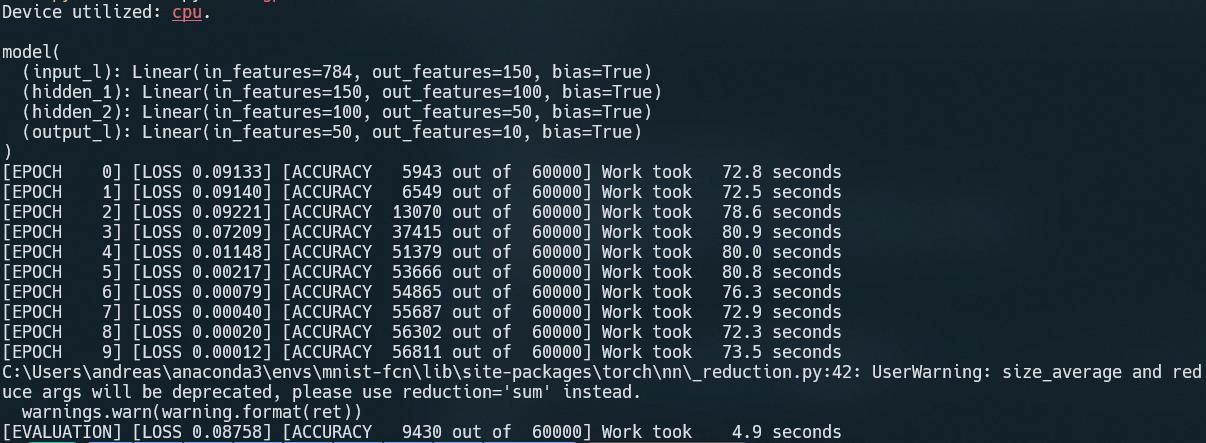
\includegraphics[width=\linewidth]{static/figures/python.PNG}
\caption{Results from the Python implementation.}
\label{fig:python}
\end{figure}

\begin{figure}[!htbp]
\centering
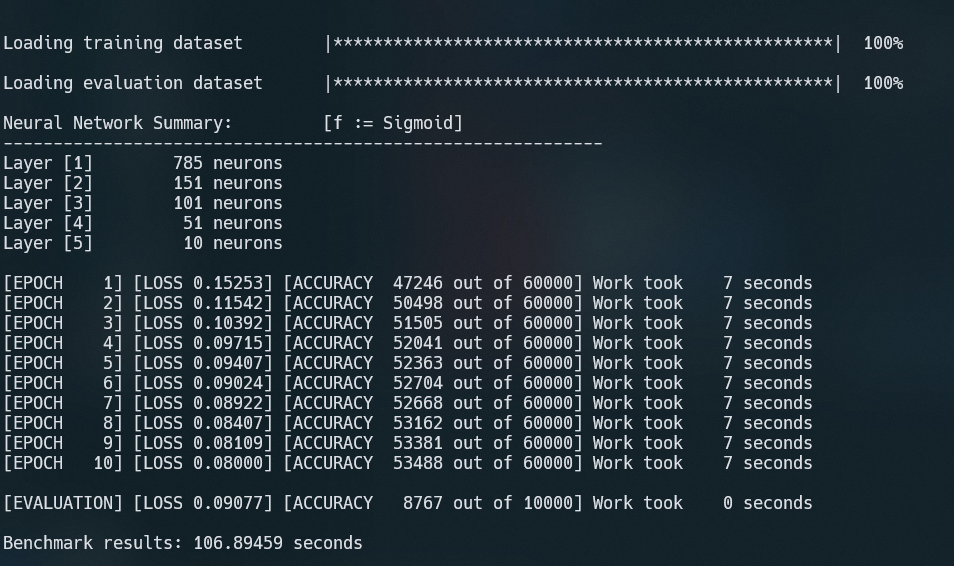
\includegraphics[width=\linewidth]{static/figures/cpp-serial.PNG}
\caption{Results from the serial \texttt{C++} implementation.}
\label{fig:cpp-serial}
\end{figure}

